%%%%%%%%%%%%%%%%%%%%%%%%%%%%%%%%%%%%%%%%%
% Beamer Presentation
% LaTeX Template
% Version 1.0 (10/11/12)
%
% This template has been downloaded from:
% http://www.LaTeXTemplates.com
%
% License:
% CC BY-NC-SA 3.0 (http://creativecommons.org/licenses/by-nc-sa/3.0/)
%
%%%%%%%%%%%%%%%%%%%%%%%%%%%%%%%%%%%%%%%%%

%----------------------------------------------------------------------------------------
%	PACKAGES AND THEMES
%----------------------------------------------------------------------------------------

\documentclass{beamer}
\geometry{papersize={171mm,96mm}}

\mode<presentation> {

% The Beamer class comes with a number of default slide themes
% which change the colors and layouts of slides. Below this is a list
% of all the themes, uncomment each in turn to see what they look like.

%\usetheme{default}
%\usetheme{AnnArbor}
%\usetheme{Antibes}
%\usetheme{Bergen}
%\usetheme{Berkeley}
%\usetheme{Berlin}
%\usetheme{Boadilla}
%\usetheme{CambridgeUS}
%\usetheme{Copenhagen}
%\usetheme{Darmstadt}
%\usetheme{Dresden}
%\usetheme{Frankfurt}
%\usetheme{Goettingen}
%\usetheme{Hannover}
%\usetheme{Ilmenau}
%\usetheme{JuanLesPins}
%\usetheme{Luebeck}
\usetheme{Madrid}
%\usetheme{Malmoe}
%\usetheme{Marburg}
%\usetheme{Montpellier}
%\usetheme{PaloAlto}
%\usetheme{Pittsburgh}
%\usetheme{Rochester}
%\usetheme{Singapore}
%\usetheme{Szeged}
%\usetheme{Warsaw}

% As well as themes, the Beamer class has a number of color themes
% for any slide theme. Uncomment each of these in turn to see how it
% changes the colors of your current slide theme.

%\usecolortheme{albatross}
%\usecolortheme{beaver}
%\usecolortheme{beetle}
%\usecolortheme{crane}
%\usecolortheme{dolphin}
%\usecolortheme{dove}
%\usecolortheme{fly}
%\usecolortheme{lily}
%\usecolortheme{orchid}
%\usecolortheme{rose}
%\usecolortheme{seagull}
%\usecolortheme{seahorse}
%\usecolortheme{whale}
%\usecolortheme{wolverine}

%\setbeamertemplate{footline} % To remove the footer line in all slides uncomment this line
%\setbeamertemplate{footline}[page number] % To replace the footer line in all slides with a simple slide count uncomment this line

%\setbeamertemplate{navigation symbols}{} % To remove the navigation symbols from the bottom of all slides uncomment this line
}


\newcommand\norm[1]{\left\lVert#1\right\rVert}
\usepackage{graphicx} % Allows including images
\usepackage{booktabs} % Allows the use of \toprule, \midrule and \bottomrule in tables
\usepackage[spanish, es-nodecimaldot]{babel}


\usepackage{mathrsfs}
\let\RSFSmathscr\mathscr  % save the meaning of \mathscr
\usepackage[scr]{rsfso}
\let\RSFSOmathscr\mathscr % save the new meaning of \mathscr
\let\mathscr\RSFSmathscr  % restore the previous meaning
\newcommand{\Laplace}{\RSFSOmathscr{L}}

\usepackage{tikz}
\def\checkmark{\tikz\fill[scale=0.4](0,.35) -- (.25,0) -- (1,.7) -- (.25,.15) -- cycle;} 

\usepackage{tabularx}
\usepackage{ragged2e}

\usepackage{amssymb}

\usepackage{sidecap}

\usepackage{listings}

\lstset{
    language=C,
    basicstyle=\ttfamily,
    numbers=left,
    numberstyle=\tiny,
    stepnumber=1,
    numbersep=5pt,
    showstringspaces=false,
    tabsize=2,
    breaklines=true,
    breakatwhitespace=true,
}

%----------------------------------------------------------------------------------------
%	TITLE PAGE
%----------------------------------------------------------------------------------------

\title[LQR]{Unidad 4.B. Control óptimo cuadrático} % The short title appears at the bottom of every slide, the full title is only on the title page

\author{Dr. Ing. Hernán Garrido} % Your name
\institute[FING-UNCUYO] % Your institution as it will appear on the bottom of every slide, may be shorthand to save space
{
Control y sistemas \\
Universidad Nacional de Cuyo, Facultad de Ingeniería \\ % Your institution for the title page
\medskip
\textit{carloshernangarrido@gmail.com} % Your email address
}
\date{Diciembre de 2023} % Date, can be changed to a custom date
\titlegraphic{
    
\includegraphics[width=0.22\textwidth]{logo_fing_uncuyo.png}
}

\begin{document}

\begin{frame}
\titlepage % Print the title page as the first slide
\end{frame}

\begin{frame}
\frametitle{Contenidos} % Table of contents slide, comment this block out to remove it
\tableofcontents % Throughout your presentation, if you choose to use \section{} and \subsection{} commands, these will automatically be printed on this slide as an overview of your presentation
\end{frame}

%---------------------------------------------------
%	PRESENTATION SLIDES
%---------------------------------------------------

%---------------------------------------------------
\section{Introducción} 
\tableofcontents[currentsection]
\begin{frame}{Introducción}
\begin{itemize}
    \item Los controladores del tipo PID, y en particular los PI son los más usados en la industria.

    \item Sin embargo, sólo sirven para plantas SISO:
    \begin{itemize}
        \item Una salida: la variable controlada
        \item Una entrada: la acción de control
    \end{itemize}

    \item En sistemas MIMO donde no haya gran acoplamiento cruzado entre entradas y salidas:

\end{itemize}

\begin{tabularx}{\textwidth}{X X}
    \begin{figure}
        \centering
        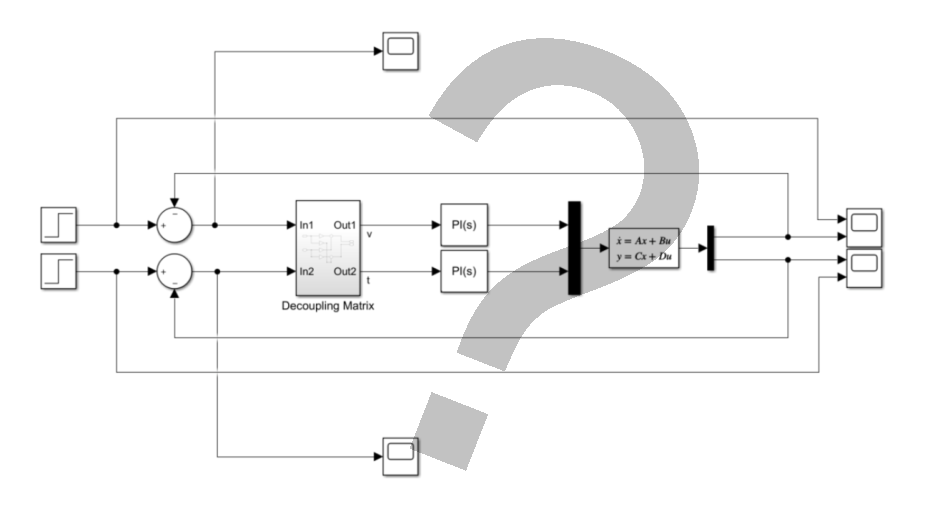
\includegraphics[width=0.4\textwidth]{MIMO_PID.pdf}
        % \caption{Caption}
        % \label{fig:enter-label}
    \end{figure}
& 
    Se pueden usar múltiples PID con cuidado:
    \begin{itemize}
        \item Simulando o experimentando en múltiples escenarios en busca de efectos no deseados.
        \item Revisando el ajuste de todos los PID, cada vez que se modifica uno de ellos o hay un cambio en la planta.
    \end{itemize}
\\
\end{tabularx}


\end{frame}


%---------------------------------------------------
\section{Repaso de control en espacio de estados y del concepto de controlabilidad} 
\tableofcontents[currentsection]
\begin{frame}{Repaso de control en espacio de estados y del concepto de controlabilidad}

... the state may be regarded as a kind of information storage or memory or accumulation of past causes. We must, of course, demand that the set of internal states $\mathbf{x}$ be sufficiently rich to carry all information about the past history of $\mathbf{x}$ to predict the effect of the past upon the future. We do not insist, however, that the state is the least such information although this is often a convenient assumption. \emph{R. E. Kalman, P. L. Falb and M. A. Arbib, Topics in Mathematical System Theory, 1969.}

\begin{figure}
    \centering
    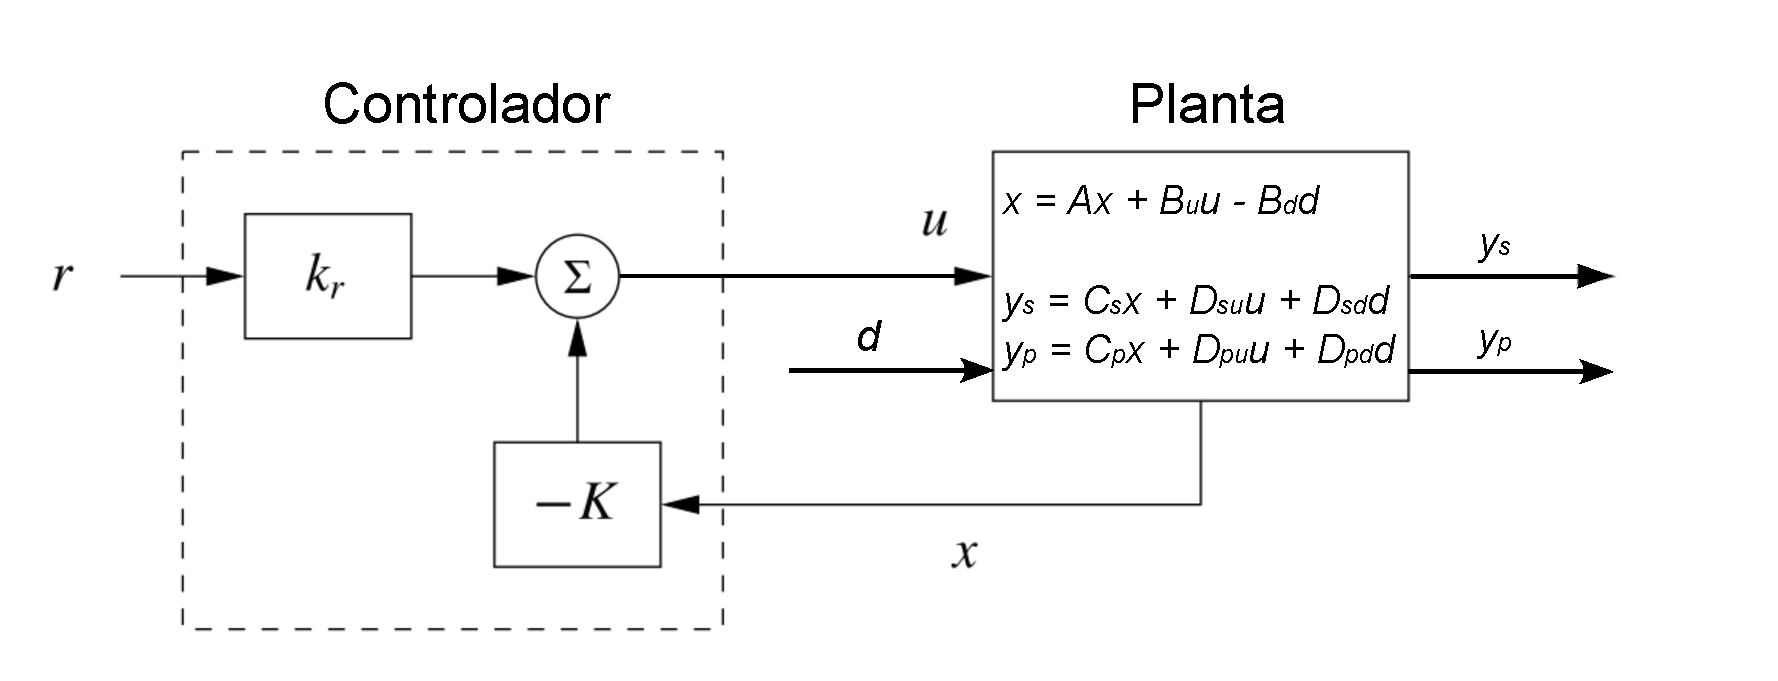
\includegraphics[width=0.82\textwidth]{MIMO_ssf.pdf}
    % \caption{Caption}
    % \label{fig:enter-label}
\end{figure}

\end{frame}

\begin{frame}{Controlabilidad y alcanzabilidad: Definiciones}
    $$\dot{\mathbf{x}}(t)=\mathbf{A}\mathbf{x}(t) + \mathbf{B_u}\mathbf{u}(t), \mathbf{d}(t) = \mathbf{0}$$

    \begin{block}{Estabilizable (\emph{stabilizability})}
        $\forall \mathbf{x}_0 \in \mathbb{R}^n, \exists \mathbf{u}: [0, \infty) \rightarrow \mathbb{R}^m: \mathbf{x}(0) = \mathbf{x}_0 \land \lim_{t \rightarrow \infty}{\mathbf{x}(t)}=\mathbf{0}$
        
        Existe una acción de control que puede llevar el estado al origen.
    \end{block}
    
    \begin{block}{Controlable (\emph{controllability})}
        $\forall \mathbf{x}_0 \in \mathbb{R}^n, \exists \mathbf{u}: [0, T] \rightarrow \mathbb{R}^m: \mathbf{x}(0) = \mathbf{x}_0 \land \mathbf{x}(T)=\mathbf{0}$
        
        Existe una acción de control, de duración finita, que puede llevar el estado al origen.
    \end{block}
    
    \begin{block}{Alcanzable (\emph{reachability})}
        $\forall (\mathbf{x}_0 \in \mathbb{R}^n, \mathbf{x}_f \in \mathbb{R}^n), \exists \mathbf{u}: [0, T] \rightarrow \mathbb{R}^m: \mathbf{x}(0) = \mathbf{x}_0 \land \mathbf{x}(T)=\mathbf{x}_f$
        
        Existe una acción de control, de duración finita, que puede llevar el estado a cualquier condición final.
    \end{block}

\end{frame}

\begin{frame}{Controlabilidad y alcanzabilidad: Test para sistemas LTI de tiempo continuo}
    $$\dot{\mathbf{x}}(t)=\mathbf{A}\mathbf{x}(t) + \mathbf{B_u}\mathbf{u}(t), \mathbf{d}(t) = \mathbf{0}$$

    $$\dot{\mathbf{x}}(t)=\mathbf{A}\mathbf{x}(t) + \mathbf{B_u}\mathbf{u}(t)$$
    
    \begin{block}{Test de alcanzabilidad}
        $$\mathbf{W}_r = \begin{bmatrix}
            \mathbf{B_u} & \mathbf{A}\mathbf{B_u} & ... & \mathbf{A}^{n-1} \mathbf{B_u}
        \end{bmatrix}_{n \times mn}$$
        Alcanzable $\iff$ $\mathrm{rank}(\mathbf{W}_r)=n$ (tiene rango completo)
    \end{block}

    \begin{block}{En general}
        alcanzabilidad $\Rightarrow$ controlabilidad $\Rightarrow$ estabilizabilidad $\Leftarrow$ estabilidad
    \end{block}

    
    \begin{block}{En sistemas LTI de tiempo continuo}
        alcanzabilidad $\iff$ controlabilidad $\Rightarrow$ estabilizabilidad $\Leftarrow$ estabilidad
    \end{block}
    
\end{frame}

\begin{frame}{Controlabilidad y alcanzabilidad: Ejemplo de inestable, no controlable pero estabilizable}
    $$
    \begin{matrix}
    \begin{bmatrix}
        \dot{x}_1(t) \\
        \dot{x}_2(t)
    \end{bmatrix}
    =
    \begin{bmatrix}
        1 & 0 \\
        0 & -1
    \end{bmatrix}
    \begin{bmatrix}
        x_1(t) \\
        x_2(t)
    \end{bmatrix}
    +
    \begin{bmatrix}
        1 \\
        0
    \end{bmatrix}
    u(t), & &
    \begin{aligned}
        &x_1(t) = x_1(0) e^t + \int_0^t{u(\tau)d\tau} \\
        &x_2(t) = x_2(0) e^{-t}
    \end{aligned}
    \end{matrix}
    $$
    
    \begin{itemize}
        \item Estabilidad
        $$\mathrm{eig}(\mathbf{A}) = \{1, -1\}
        \Rightarrow \Re(1) > 0 \Rightarrow \mathbf{A}  ~\mathrm{inestable}$$

        \item Controlabilidad
        $$\mathbf{W}_r = \begin{bmatrix}
            \begin{bmatrix}
                1 \\
                0
            \end{bmatrix}
            &
            \begin{bmatrix}
                1 & 0 \\
                0 & -1
            \end{bmatrix}
            \begin{bmatrix}
                1 \\
                0
            \end{bmatrix}
        \end{bmatrix}
        =
        \begin{bmatrix}
            1 & 1 \\
            0 & 0
        \end{bmatrix}
        \Rightarrow
        \mathrm{rank}(\mathbf{W}_r)=1<2=n
        \Rightarrow
        (\mathbf{A}, \mathbf{B_u})~\mathrm{no~controlable}
        $$

        \item Estabilizabilidad
        $$
        \begin{matrix}
            u(t) = -2 x_1(t) \\
            \dot{x}_1(t) = x_1(t) + u(t) = -x_1(t)
        \end{matrix}
        \Rightarrow
        \begin{aligned}
            &x_1(t) = x_1(0) e^{-t} \\
            &x_2(t) = x_2(0) e^{-t}
        \end{aligned}
        \Rightarrow
        \begin{matrix}
            \forall \mathbf{x}_0 = \mathbf{x}(0)\\
            \lim_{t \rightarrow \infty}{\mathbf{x}(t)}=\mathbf{0} 
        \end{matrix}
        \Rightarrow
        (\mathbf{A}, \mathbf{B_u})~\mathrm{estabilizable}
        $$
        Corolario: Si todos los modos no controlables son estables, el sistema es estabilizable.
    \end{itemize}
    
    
\end{frame}

\begin{frame}{Controlabilidad y alcanzabilidad: Ejemplo de controlable pero no alcanzable}
    \begin{itemize}
        \item En tiempo discreto
        $$
        \begin{matrix}
            \begin{bmatrix}
                x_1 \\
                x_2
            \end{bmatrix}_{k+1}
            =
            \begin{bmatrix}
                1 & 0\\
                0 & 0
            \end{bmatrix}
            \begin{bmatrix}
                x_1 \\
                x_2
            \end{bmatrix}_{k}
            +
            \begin{bmatrix}
                1 \\
                0
            \end{bmatrix}    u_k
            & & &
            \begin{aligned}
                & x_1[k+1] = x_1[k] + u[k] \\
                & x_2[k+1] = 0
            \end{aligned}
        \end{matrix}
        $$
    
        \begin{itemize}
            \item Alcanzabilidad
            $$\mathbf{W}_r = \begin{bmatrix}
                \begin{bmatrix}
                    1 \\
                    0
                \end{bmatrix}
                &
                \begin{bmatrix}
                    1 & 0\\
                    0 & 0
                \end{bmatrix}
                \begin{bmatrix}
                    1 \\
                    0
                \end{bmatrix}
            \end{bmatrix}
            =
            \begin{bmatrix}
                1 & 1\\
                0 & 0
            \end{bmatrix}
            \Rightarrow
            \mathrm{rank}(\mathbf{W}_r)=1<2=n
            \Rightarrow
            (\mathbf{A_d}, \mathbf{B_u})~\mathrm{no~alcanzable}
            $$ 
            \item Controlabilidad
            $$u[k] = -x_1[k]
            \Rightarrow
            \begin{aligned}
                & x_1[k+1] = x_1[k] - x_1[k] = 0 \\
                & x_2[k+1] = 0
            \end{aligned}\Rightarrow
            \begin{aligned}
                \forall \mathbf{x}_0 = \mathbf{x}[0] \\
                \mathbf{x}[1] = \begin{bmatrix}
                    0 \\
                    0
                \end{bmatrix}
            \end{aligned}
            \Rightarrow
            (\mathbf{A_d}, \mathbf{B_u})~\mathrm{controlable}
            $$
        \end{itemize}
    \item En tiempo continuo (sistemas LTI):
    
        Controlable $\iff$ Alcanzable
    \end{itemize}
\end{frame}

%---------------------------------------------------
\section{Control en espacio de estados} 
\tableofcontents[currentsection]
\begin{frame}{Control en espacio de estados}
    \begin{itemize}
        \item Control para estabilizar una planta
        \begin{itemize}
            \item Objetivo: Hacer que $\mathbf{x}(t) \rightarrow \mathbf{0}$ cuando $\mathbf{r}(t)=\mathbf{0}$ y las perturbaciones son nulas.
            \item Implementación: Con realimentación completa del vector de estado
            $$
            \begin{cases}
                \mathbf{\dot{x}}(t) = \mathbf{A} \mathbf{x}(t) + \mathbf{B_u} \mathbf{u}(t) \\
                \mathbf{y_p}(t) = \mathbf{C_p} \mathbf{x}(t)
            \end{cases}
            \Rightarrow \mathbf{X}(s) = (s\mathbf{I} - \mathbf{A})^{-1} \mathbf{B_u}\mathbf{U}(s)$$
            
            $$\mathbf{u}(t) = -\mathbf{K}\mathbf{x}(t) \Rightarrow \mathbf{\dot{x}} = (\mathbf{A} - \mathbf{K B_u}) \mathbf{x}$$
            $\mathbf{A}$ puede ser inestable (hay raíces de $|s \mathbf{I} - \mathbf{A}| = 0$ tienen parte real positiva), pero se puede elegir $\mathbf{K}$ para que $\mathbf{A} - \mathbf{K B_u}$ sí lo sea (todas las raíces de $|s\mathbf{I} - (\mathbf{A} - \mathbf{K}\mathbf{B}_\mathrm{u})|$ tengan parte real negativa).
        \end{itemize}  
        
        \item Control para regular una planta estabilizada
        \begin{itemize}
            \item Objetivo: Hacer que $\mathbf{y_p}(t) \rightarrow \mathbf{r}(t)$ cuando $\mathbf{x}(t)=\mathbf{0}$ y las perturbaciones sean nulas.
            \item Implementación:
            Sistema a lazo cerrado con ganancia $\mathbf{I}$, al menos para $t \rightarrow \infty, s \rightarrow 0$
            $$\mathbf{u}(t) = \mathbf{k_r}\mathbf{r}(t) -\mathbf{K}\mathbf{x}(t) \Rightarrow \mathbf{U}(s) = \mathbf{k_r}\mathbf{R}(s) -\mathbf{K}\mathbf{X}(s)$$
            $$s \mathbf{X}(s) = \mathbf{A}\mathbf{X}(s) + \mathbf{B_u} (\mathbf{k_r}\mathbf{R}(s) -\mathbf{K}\mathbf{X}(s)) = \mathbf{A}\mathbf{X}(s) - \mathbf{B_u} \mathbf{K}\mathbf{X}(s) + \mathbf{B_u} \mathbf{k_r}\mathbf{R}(s)$$
            $$(s\mathbf{I} - (\mathbf{A} - \mathbf{B_u K})) \mathbf{X}(s) = \mathbf{B_u k_r R}(s) \Rightarrow \mathbf{Y_p}(s) \mathbf{R}^{-1}(s) = \frac{\mathbf{Y_p}(s)}{\mathbf{R}(s)} = \mathbf{C_p} (s\mathbf{I} - (\mathbf{A} - \mathbf{B_u K}))^{-1} \mathbf{B_u k_r}$$
        \end{itemize}
    \end{itemize}
    
\end{frame}

%---------------------------------------------------
\section{Cálculo de ganancia de realimentación y ganancia de referencia} 
\tableofcontents[currentsection]
\begin{frame}{Ganancia de realimentación}
Asignación de polos:
Encontrar $\mathbf{K}$ tal que las raíces de
$$|s\mathbf{I} - (\mathbf{A - KB_u})| = 0$$ sean prescritas como $s_0, s_1, ..., s_{n-1}$

\begin{block}{Método de Ackermann}
    Si el par $\mathbf{A}, \mathbf{B_u}$ es controlable, se puede plantear un sistema de ecuaciones donde las ganancias (elementos de $\mathbf{K}$) son incógnitas. Se puede resolver directamente con Matlab mediante las funciones \emph{acker} o \emph{place} de Matlab o del paquete control en python (pip install control).
\end{block}

\end{frame}

\begin{frame}{Ganancia de referencia (ganancia de pre-alimentación)}
Ganancia para seguir una referencia, al menos para $t \rightarrow \infty$: Encontrar $\mathbf{k_r}$ tal que
$$\left. \frac{\mathbf{Y_p}(s)}{\mathbf{R}(s)} \right|_{s=0} = \left. \mathbf{C_p} (s\mathbf{I} - (\mathbf{A} - \mathbf{B_u K}))^{-1} \mathbf{B_u k_r} \right|_{s=0} = \mathbf{I}$$
$$\mathbf{k_r} = (\mathbf{C_p}(0 \cdot \mathbf{I} - (\mathbf{A} - \mathbf{B_u K}))^{-1} \mathbf{B_u})^{-1}$$

\begin{block}{Método de la ganancia en régimen estacionario de la planta estabilizada}
    La acción de control resultante es:
    $$\mathbf{u}(t) = -\mathbf{Kx}(t) + \mathbf{k_r r}(t)$$
    donde la ganancia de pre-alimentación $\mathbf{k_r}$ se calcula como:
    $$\mathbf{k_r} =  -(\mathbf{C_p} (\mathbf{A} - \mathbf{B_u K})^{-1} \mathbf{B_u})^{-1}$$
    para lo cual $\mathbf{B_u}$ debe tener tantas columnas como filas tenga $\mathbf{C_p}$. Es decir, debe haber al menos un actuador por cada variable que se quiera seguir. 
\end{block}

\end{frame}


%---------------------------------------------------
\section{Ruido y perturbaciones} 
\tableofcontents[currentsection]
\begin{frame}{Ruido y perturbaciones}
\begin{block}{Ruido en los sensores}
    Se modelan normalmente en forma aditiva:
    $$\mathbf{y_s}(t) = \mathbf{C_s}\mathbf{x}(t) + \mathbf{n}(t)$$
    donde $\mathbf{n}(t)$ debe ser consistente con las especificaciones del fabricante del sensor y demás particularidades de la aplicación. Ejemplos: cuantización, ruido blanco, ruido de línea, de derivada numérica.
\end{block}

\begin{block}{Perturbaciones sobre la planta}
    Se modelan normalmente en forma aditiva:
    $$\mathbf{\dot{x}}(t) = \mathbf{A} \mathbf{x}(t) + \mathbf{B_u} \mathbf{u}(t) + \mathbf{B_d} \mathbf{d}(t)$$
    donde $\mathbf{d}(t)$ representa todas las acciones que excitan a la planta y no son definidas por el controlador. Ejemplos: gravedad, ruido mecánico, viento, sismo, vandalismo.
\end{block}

\end{frame}

%---------------------------------------------------
\section{Acción integral} 
\tableofcontents[currentsection]
\begin{frame}{Acción integral}
Debido a:
\begin{itemize}
    \item errores en la calibración de los parámetros del modelo de la planta
    \item perturbaciones con componente de estado estacionario
    \item ruidos con componente de estado estacionario
\end{itemize}
puede aparecer \emph{error de estado estacionario} entre $\mathbf{y_p}(t)$ y $\mathbf{r}(t)$.

\begin{block}{Solución}
    Aumentar el vector de estado $\mathbf{x}(t)$ con una variable $z_i(t)$ por cada referencia a seguir, tal que:
    $$\dot{\mathbf{z}}(t) = \mathbf{y_p}(t) - \mathbf{r}(t)$$
    es decir, que el nuevo estado incluye la integral del error de cada referencia a seguir.
\end{block}
\end{frame}


\begin{frame}{Acción integral}
    El sistema aumentado es:
    $$\mathbf{\dot{x}}(t) = \mathbf{A} \mathbf{x}(t) + \mathbf{B_u} \mathbf{u}(t) + \mathbf{B_d} \mathbf{d}(t)$$
    $$\dot{\mathbf{z}}(t) = \mathbf{y_p}(t) - \mathbf{r}(t) = \mathbf{C_p x}(t) - \mathbf{r}(t)$$
    que en forma matricial resulta:
        $$
    \begin{bmatrix}
    \mathbf{\dot{x}}(t) \\
    \dot{\mathbf{z}}(t)
    \end{bmatrix} = 
    \underbrace{\begin{bmatrix}
    \mathbf{A} & \mathbf{0} \\
    \mathbf{C_p} & \mathbf{0}
    \end{bmatrix}}_{\mathbf{A_{\text{aug}}}}
    \begin{bmatrix}
    \mathbf{x}(t) \\
    \mathbf{z}(t)
    \end{bmatrix} + 
    \underbrace{\begin{bmatrix}
    \mathbf{B_u} \\
    \mathbf{0}
    \end{bmatrix}}_{\mathbf{B_{\text{aug}}}}
    \mathbf{u}(t) + 
    \underbrace{\begin{bmatrix}
    \mathbf{B_d} \\
    \mathbf{0}
    \end{bmatrix}}_{\mathbf{B_{d,\text{aug}}}}
    \mathbf{d}(t) + 
    \underbrace{\begin{bmatrix}
    \mathbf{0} \\
    -\mathbf{I}
    \end{bmatrix}}_{\mathbf{B_{r}}}
    \mathbf{r}(t)
    $$
    
    \begin{itemize}
        \item Nueva variable de estado: $\mathbf{z}(t) = \int (\mathbf{y_p}(t) - \mathbf{r}(t)) \mathrm{d}t$
        \item Matriz aumentada $\mathbf{A_{\text{aug}}}$ de dimensión $(n+p)\times(n+p)$
        \item Permite eliminar error en régimen permanente
    \end{itemize}

\end{frame}


\begin{frame}{Diseño del controlador integral (con seguimiento de referencia)}
    Ley de control para estabilizar y controlar error en estado estacionario: 
    $$\mathbf{u}(t) = -\mathbf{K}\mathbf{x}(t) - \mathbf{K_i}\mathbf{z}(t) = -\begin{bmatrix}\mathbf{K} & \mathbf{K_i}\end{bmatrix}\begin{bmatrix}\mathbf{x}(t) \\ \mathbf{z}(t)\end{bmatrix}$$
    
    donde
    $$ \mathbf{K_{\text{aug}}} = \begin{bmatrix}\mathbf{K} & \mathbf{K_i}\end{bmatrix} \quad \text{ y }  \quad \mathbf{x}_\text{aug} = \begin{bmatrix}\mathbf{x}(t) \\ \mathbf{z}(t)\end{bmatrix} \quad \text{ con lo cual: } \quad \mathbf{u}(t) = -\mathbf{K_{\text{aug}}}\mathbf{x}_\text{aug}$$
    
    \textbf{Paso 1:} Obtener $\mathbf{K_{\text{aug}}}$ mediante:
    \begin{itemize}
        \item Asignación de polos al sistema aumentado, cuyo polinomio característico es $\det(s\mathbf{I} - \mathbf{A_{\text{aug}}} + \mathbf{B_{\text{aug}}}\mathbf{K_{\text{aug}}}) = 0$, o LQR
    \end{itemize}

    \textbf{Paso 2:} Extraer $\mathbf{K}$ y $\mathbf{K_i}$ de $\mathbf{K_{\text{aug}}}$

    \textbf{Paso 3:} Calcular la ganancia de pre-alimentación mediante: $\mathbf{k_r} =  -(\mathbf{C_p} (\mathbf{A} - \mathbf{B_u K})^{-1} \mathbf{B_u})^{-1}$

    \begin{block}{Ley de control completa}
        $$\mathbf{u}(t) = -\mathbf{K x}(t) - \mathbf{K_i z}(t) + \mathbf{k_r r}(t)$$
    \end{block}
    

\end{frame}


%---------------------------------------------------
\section{Regulador lineal cuadrático (LQR)} 
\tableofcontents[currentsection]
\begin{frame}{Regulador lineal cuadrático (LQR): Motivación}
Motivación:

La ubicación de los polos del polinomio característico a lazo cerrado (mediante \emph{acker} o \emph{place}):
\begin{itemize}
    \item Permite definir la definir la dinámica \emph{discrecionalmente} a partir de especificaciones temporales.
    \item Pero, en la práctica siempre se debe chequear que las acciones de control sean \emph{económicamente} razonables.
    \begin{itemize}
        \item Esto lleva a muchas iteraciones de diseño en proyectos reales.
    \end{itemize} 
    \item Además, no ofrece discrecionalidad sobre la autoridad de control en cada variable, grado de libertad o modo dinámico.
\end{itemize}

Solución:

Plantear un problema de optimización que pondere:
\begin{itemize}
    \item Autoridad sobre cada variable de estado, o combinaciones entre ellas. Ejemplos
    \begin{itemize}
        \item posición, velocidad, integral del error
        \item distancia entre efectores
    \end{itemize}
    \item Intensidad de las acciones de control, o combinaciones entre ellas:
    \begin{itemize}
        \item voltaje, corriente
        \item potencia
    \end{itemize}
\end{itemize}
\end{frame}


\begin{frame}{Regulador lineal cuadrático (LQR): Formulación}

Minimizamos la función de costo cuadrático:
\begin{equation}
\tilde{J} = \int_{0}^{\infty} \left( \mathbf{x}^T\mathbf{Q}_x\mathbf{x} + \mathbf{u}^T\mathbf{Q}_u\mathbf{u} \right) \mathrm{d}t
\label{eq:costo_quadratico}
\end{equation}

donde:
\begin{itemize}
\item $\mathbf{Q}_x \in \mathbb{R}^{n \times n}$, $\mathbf{Q}_x \succeq 0$ (matriz simétrica y semidefinida positiva)
\item $\mathbf{Q}_u \in \mathbb{R}^{m \times m}$, $\mathbf{Q}_u \succ 0$ (matriz simétrica y definida positiva)
\item $\mathbf{x} \in \mathbb{R}^n$: Vector de estados
\item $\mathbf{u} \in \mathbb{R}^m$: Vector de acciones de control
\end{itemize}

Esta formulación establece un balance entre:
\begin{itemize}
\item \textbf{Regulación de estados}: $\mathbf{x}^T\mathbf{Q}_x\mathbf{x}$ penaliza las desviaciones del estado respecto al origen
\item \textbf{Economía de control}: $\mathbf{u}^T\mathbf{Q}_u\mathbf{u}$ penaliza el uso excesivo de acciones de control
\end{itemize}

\end{frame}



\begin{frame}{Regulador lineal cuadrático (LQR): Interpretación}

\begin{equation}
J = \int_{0}^{\infty} \left( \mathbf{x}^T\mathbf{Q}_x\mathbf{x} + \mathbf{u}^T\mathbf{Q}_u\mathbf{u} \right) \mathrm{d}t
\label{eq:costo_quadratico}
\end{equation}

La matriz $\mathbf{K}$ que minimiza $J$ aplicando la ley de control $\mathbf{u}(t) = -\mathbf{K x}(t)$ se encuentra resolviendo una ecuación de Ricatti. En la práctica simplemente usamos la función \emph{lqr} de Matlab o del paquete \emph{control} en python.\footnote{Se puede trabajar con $\mathbf{x}_\text{aug}$, generando $\mathbf{Q}_{x\text{aug}}$, para encontrar $\mathbf{K}_\text{aug}$}

\textbf{Lo importante es definir correctamente $\mathbf{Q}_u$ y $\mathbf{Q}_x$:}

\begin{equation}
\mathbf{x}^T\mathbf{Q}_x\mathbf{x} = 
\begin{bmatrix} x_1 & x_2 & x_3 \end{bmatrix}
\begin{bmatrix} q_{11} & q_{12} & q_{13} \\ q_{12} & q_{22} & q_{23} \\ q_{13} & q_{23} & q_{33} \end{bmatrix}
\begin{bmatrix} x_1 \\ x_2 \\ x_3 \end{bmatrix} =
q_{11}x_1^2 + 2q_{12}x_1x_2 + 2q_{13}x_1x_3 + q_{22}x_2^2 + 2q_{23}x_2x_3 + q_{33}x_3^2
\end{equation}

\begin{equation}
\mathbf{u}^T\mathbf{Q}_u\mathbf{u} = 
\begin{bmatrix} u_1 & u_2 \end{bmatrix}
\begin{bmatrix} r_{11} & r_{12} \\ r_{12} & r_{22} \end{bmatrix}
\begin{bmatrix} u_1 \\ u_2 \end{bmatrix} =
r_{11}u_1^2 + 2r_{12}u_1u_2 + r_{22}u_2^2
\end{equation}

\end{frame}


\begin{frame}{Regulador lineal cuadrático (LQR): Técnicas para elegir $\mathbf{Q}_u$ y $\mathbf{Q}_x$}
\begin{block}{Regla de Bryson (Bryson y Ho, 1975)}
\[
\mathbf{Q_x} = \begin{bmatrix}
1/x_{1\text{typ}}^2 & 0 & \cdots & 0 \\
0 & 1/x_{2\text{typ}}^2 & \cdots & 0 \\
\vdots & \vdots & \ddots & \vdots \\
0 & 0 & \cdots & 1/x_{n\text{typ}}^2
\end{bmatrix}
\]

\[
\mathbf{Q_u} = \begin{bmatrix}
1/u_{1\text{typ}}^2 & 0 & \cdots & 0 \\
0 & 1/u_{2\text{typ}}^2 & \cdots & 0 \\
\vdots & \vdots & \ddots & \vdots \\
0 & 0 & \cdots & 1/u_{n\text{typ}}^2
\end{bmatrix}
\]

\end{block}

\end{frame}



\begin{frame}{Regulador lineal cuadrático (LQR): Técnicas para elegir $\mathbf{Q}_u$ y $\mathbf{Q}_x$}
\begin{block}{Regla de Bryson (Bryson y Ho, 1975) adaptable}
$$\mathbf{y_p} = \mathbf{C_p} \mathbf{x}$$

$$
\mathbf{Q_p} = \begin{bmatrix}
1/y_{p1\text{typ}}^2 & 0 & \cdots & 0 \\
0 & 1/y_{p2\text{typ}}^2 & \cdots & 0 \\
\vdots & \vdots & \ddots & \vdots \\
0 & 0 & \cdots & 1/y_{pn\text{typ}}^2
\end{bmatrix}
$$

$$\mathbf{Q_x} = \mathbf{C_p}^\intercal \mathbf{Q_p} \mathbf{C_p}$$

La matriz $\mathbf{C_p}$ permite construir cualquier combinación lineal de los estados.

\end{block}

\end{frame}


\begin{frame}{Regulador lineal cuadrático (LQR): Regla de Bryson adaptable}

\textbf{Ejemplo 1:} Dado $\mathbf{x} = [x_1, x_2]^\intercal$, minimizar $|x_1 + x_2|$:

\[
\mathbf{y_p} = \mathbf{C_p} \mathbf{x} = y_p = x_1 + x_2 = \begin{bmatrix}
        1 & 1
    \end{bmatrix}
    \begin{bmatrix}
        x_1 \\ x_2
    \end{bmatrix}
\]
\[
\mathbf{C_p} = \begin{bmatrix}
        1 & 1
    \end{bmatrix}, \quad
\mathbf{Q_p} = \begin{bmatrix}
        q_p
    \end{bmatrix}
\]
\[
\mathbf{Q}_x = \mathbf{C_p}^\intercal \mathbf{Q_p} \mathbf{C_p} = \begin{bmatrix}
        1 \\ 1
    \end{bmatrix}
    \begin{bmatrix}
        q_p
    \end{bmatrix}
    \begin{bmatrix}
        1 & 1
    \end{bmatrix} = \begin{bmatrix}
        q_p & q_p \\
        q_p & q_p
    \end{bmatrix}
\]

\[
\mathbf{x}^\intercal \mathbf{Q}_x \mathbf{x} = \begin{bmatrix}
        x_1 & x_2
    \end{bmatrix}
    \begin{bmatrix}
        q_p & q_p \\
        q_p & q_p
    \end{bmatrix}
    \begin{bmatrix}
        x_1 \\ x_2
    \end{bmatrix}
= q_p x_1^2 + q_p x_1 x_2 + q_p x_2 x_1 + q_p x_2^2
\]
\[
= q_p (x_1^2 + 2 x_1 x_2 + x_2^2)
= q_p (x_1 + x_2)^2
\]

\[
J = \int_0^\infty \left( \mathbf{x}^\intercal \mathbf{Q}_x \mathbf{x} + \mathbf{u}^\intercal \mathbf{Q}_u \mathbf{u} \right) dt = \int_0^\infty \left( q_p (x_1 + x_2)^2 + \mathbf{u}^\intercal \mathbf{Q}_u \mathbf{u} \right) dt
\]

\end{frame}



\begin{frame}{Regulador lineal cuadrático (LQR): Regla de Bryson adaptable}

\textbf{Ejemplo 2:} Dado $\mathbf{x} = [x_1, x_2]^\intercal$, minimizar \(|x_1| + |x_2|\):

\[
\mathbf{y_p} = \mathbf{C_p} \mathbf{x} = \begin{bmatrix}
        x_1 \\ x_2
    \end{bmatrix}
\]
\[
\mathbf{C_p} = \begin{bmatrix}
        1 & 0 \\
        0 & 1
    \end{bmatrix}, \quad
\mathbf{Q_p} = \begin{bmatrix}
        q_p & 0 \\
        0 & q_p
    \end{bmatrix}
\]
\[
\mathbf{Q}_x = \mathbf{C_p}^\intercal \mathbf{Q_p} \mathbf{C_p} = \begin{bmatrix}
        1 & 0 \\
        0 & 1
    \end{bmatrix}
    \begin{bmatrix}
        q_p & 0 \\
        0 & q_p
    \end{bmatrix}
    \begin{bmatrix}
        1 & 0 \\
        0 & 1
    \end{bmatrix} = \begin{bmatrix}
        q_p & 0 \\
        0 & q_p
    \end{bmatrix}
\]

\[
\mathbf{x}^\intercal \mathbf{Q}_x \mathbf{x} = \begin{bmatrix}
        x_1 & x_2
    \end{bmatrix}
    \begin{bmatrix}
        q_p & 0 \\
        0 & q_p
    \end{bmatrix}
    \begin{bmatrix}
        x_1 \\ x_2
    \end{bmatrix}
= q_p x_1^2 + q_p x_2^2
\]

\[
J = \int_0^\infty \left( \mathbf{x}^\intercal \mathbf{Q}_x \mathbf{x} + \mathbf{u}^\intercal \mathbf{Q}_u \mathbf{u} \right) dt = \int_0^\infty \left( q_p (x_1^2 + x_2^2) + \mathbf{u}^\intercal \mathbf{Q}_u \mathbf{u} \right) dt
\]

\end{frame}


\begin{frame}{Ejemplo práctico}
    \begin{figure}
        \centering
        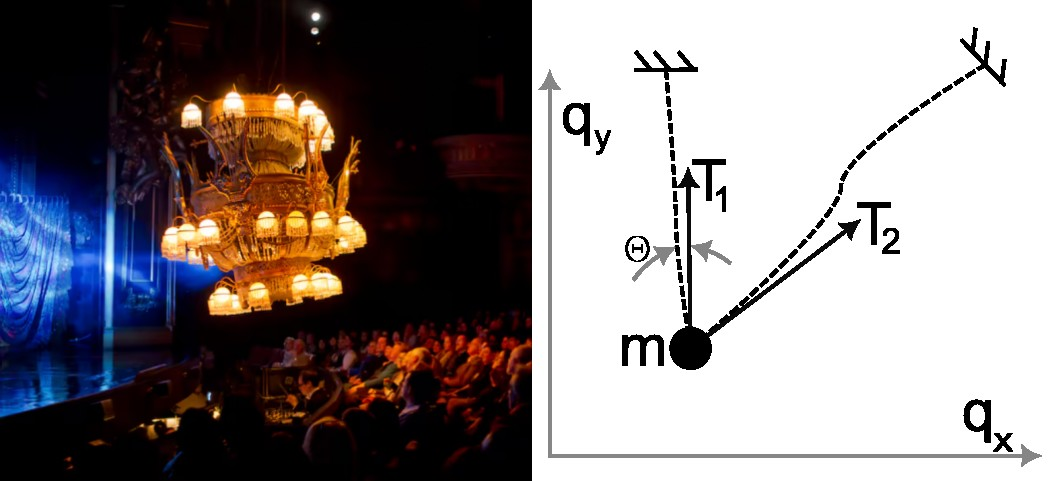
\includegraphics[width=0.9\linewidth]{opera_phantom.jpg}
        \caption{La lámpara del Fantasma de la Ópera}
    \end{figure}
\end{frame}

\begin{frame}{Bibliografía}
    \begin{enumerate}
        \item Astrom, K. J., and Murray, R. M. (2008). Feedback Systems. Princeton University Press.
        \item Ogata, K. (2010). Modern control engineering (5th ed.). Prentice Hall.
    \end{enumerate}
\end{frame}


\end{document}